\chapter{Introduction}
	\section{Indoor Stadium }
\subsection{Development stage}
Development stage of the indoor stadum is divided into three different stages :
\begin{enumerate}
	\item Idea stage
	\item Experiment stage
	\item Application stage.
\end{enumerate}	

In the initial phase of our project we have visited Jimmy George Memorial Indoor Stadium at Trivandrum and details of a standard Indoor stadium is analyzed and listed out. Afterwards initial site investigation was carried out in order for the location of indoor stadium. Drawings of the indoor stadium were developed according to the standards of Sports Authority of India (SAI).
By using software structural models were developed, designed and analyzed. To perform an accurate analysis a structural engineer must determine such information as structural loads, geometry, support conditions, material properties. The results of such an analysis typically include support reactions, stresses and displacements. This information is then compared to criteria that indicate the conditions of failure. Advanced structural analysis may examine dynamic response, stability and non-linear behavior.
The software’s used for the completion of project include Auto CAD 2016 for architectural drawings, SAP 2000 for designing and analyzing the structure and MS word, Excel for preparing documents and spreadsheets for documentation and calculation

\section{Need for Indoor Stadium}
The availability and quality of Sports Infrastructure is essential for a country to achieve success in
the global sports arena. The facilities encourage children and young adults to actively take part in
sporting activities and equip them with the skills to succeed and shine in an international forum.
\\The sporting culture in India has not been impressive in the past and this scenario can be attributed
majorly to lack of good infrastructure, among other factors. The non-availability of infrastructure
poses a major impediment to the development of sports in the country.
\\ Taking into account the current scenario and the need to
empower the youth of its state to compete globally, the Government has laid a
strong emphasis on providing world class sports infrastructure to its aspiring population. As part
of this, the government has proposed to build world-class integrated sports complexes in the state
to achieve its objective .\\


\section{Project Background}
The Project objective is to develop an integrated sports complex in College of Engineering Pathanapuram under Sports Authority of India.\\
The state of Kerala is determined to develop an Integrated Sports Complexes that will
encourage sporting activities and healthy lifestyle in the region. The facility would act as a venue
for  sporting events and would also promote sports/sportspersons across
the region by means of academies. The local population would substantially benefit from this
complex as it would encourage them to enrol in sports via membership schemes and thus promote
healthy living. People with inclination to take up professional sports would have adequate
opportunities to get trained via experienced and reputed coaches.\\
Based on the preliminary assessment that is subject to modification during future stages of bidding,
it is envisaged that the sporting complex facility would spread across 2400 sq. m of land and would
include arenas to host : 
\begin{enumerate}
	\item Professional sports leagues
	\item Student/University activities
	\item Sports Academies, Training institutions and Camps
	\item Concerts \& Shows
	\item Corporate events
	\item Commercial establishments
	\item Food and Beverage Facilities
	\item Entertainment and Leisure activities
\end{enumerate}

\section{	Indoor Stadium facilities}	
\begin{enumerate}
	\item Indoor Stadium  – 1200 gallery capacity	\item  Badminton Courts - (To be interchangeably used as Badminton/Volleyball courts ) – 6 Nos	\item Basket ball court
	\item Table Tennis
	\item  Gymnasium – 1 No
	\item Meditaion Centre
	\item  Other facilities like store rooms,wash rooms,rest rooms.
	\item  Parking area
\end{enumerate}

\section{Location}
The college is located at Elikkattoor near Piravanthoor junction on the side of Punalur-Muvattupuzha road (Between Punalur and Pathanapuram) which is 7 kms from Punalur and 8 kms from Pathanapuram.

Nearest Railway Stations : Punalur,Kollam,Kayamkulam,Chengannur

Nearest Bus Stations : Punalur,Pathanapuram.


The project involves planning, design and estimation of an indoor stadium for College of Engineering, Pathanapuram with the help of structural design software SAP 2000, AutoCAD 2016. The components of the structures designed using SAP 2000 are beams, columns, slabs, stair cases, retaining walls, foundations etc. In the initial phase of our project we have visited Jimmy George Memorial Indoor Stadium at Trivandrum and details of a standard Indoor stadium is analyzed and listed out. Afterwards initial site investigation was carried out in order for the location of indoor stadium. Drawings of the indoor stadium were developed according to the standards of sporting facilities.
By using software structural models were developed, designed and analyzed. To perform an accurate analysis a structural engineer must determine such information as structural loads, geometry, support conditions, material properties. The results of such an analysis typically include support reactions, stresses and displacements. This information is then compared to criteria that indicate the conditions of failure. Advanced structural analysis may examine dynamic response, stability and non-linear behavior.
The software’s used for the completion of project include Auto CAD 2016 for architectural drawings, SAP 2000 for designing and analyzing the structure and MS word, Excel for preparing documents and spreadsheets for documentation and calculation. 
\\The aim of the project is to plan, design and estimate an indoor stadium for college of engineering, Pathanapuram. The aim of design is achievement so that the structure will perform satisfactorily during their intended life. With an appropriate degree of safety, they should sustain all the loads and deformations of normal construction and use and have adequate durability and resistance to the effects of seismic and wind. Structure and structural elements shall normally be designed by Limit state method. Account should be taken of accepted theories, experiment and experience and the need to design for durability. Design, including design for durability, construction and use in service should be considered as a whole. The realization of design objectives requires compliance with clearly defined standards for materials, production, workmanship and also maintenance and use of structure in service. 
The design of the building is dependent upon the minimum requirements as prescribed in the India standard Codes. The minimum requirements pertaining to the structural safety of building are being covered by way of laying down minimum design loads which have to be assumed for dead loads, imposed loads, and other external loads, the structure would be required to bear. Strict conformity to loading standards recommended in these codes, it is hoped, will not only ensure the structural safety of the buildings which are being designed.
\section{Loading}
The structure will be analyzed for various loads and load combinations as per IS standards. The various loads considered should be acting on the structure are dead loads, live loads due to imposed elements , wind loads and seismic loads due to earthquake motions. For the various load considered, load combinations were provided and analyzed for results. The loads on each structural elements were considered as per IS standards.\\
Loading weights and pressures used in the SAP model were calculated in accordance 
with Indian Standard Building Codes. These loads were calculated over an area and 
distributed into the structural beam, column, and shear wall components. \\
\subsection{Dead Loads}
All permanent constructions of the structure form the dead loads. The dead load comprises of the weights of walls, partition floor finishes, false ceilings, false floors and the other permanent constructions in the buildings. The dead loads may be calculated from the dimensions of various members and their unit weights. The unit weights of common burnt clay bricks, plain concrete and reinforced concrete made with sand and gravel or crushed natural stone aggregate may be taken as per IS 875 (Part 1) -1987.
\subsection{Imposed Loads}
Imposed load is produced by the intended or occupancy of the building including the weight of the movable partitions, distributed and concentrated; loads, loads due to impact and vibration and dust loads. According to the Kerala Municipality BUIDING RULES 1999 (kmbr) . Imposed loads due not includes loads due to wind , seismic activity, snow and load imposed due to the temperature changes to which the structure will be subjected to creep and shrinkage of the structure , the differential settlement to which the structure may undergo.
\subsection{Wind Load}
Wind is air in motion relative to the surface of earth. The primary cause of wind is traced to earth’s rotation and difference in terrestrial radiation. The radiation effects are primarily responsible for convection either upwards or downwards. The wind generally blows horizontal to the ground at high wind speeds. Since vertical components of atmospheric motion are relatively small, the term ‘wind’ denotes almost exclusively the horizontal wind, vertical winds are always identified as such. The wind speed is assessed with the aid of anemometers or anemographs which are installed at metrological observatories at heights generally varying from 10 to 30 meters above ground. The wind load is calculated as per IS: 875 (Part 3) 1987.\\
Design Wind Speed (Vz)\\
The basic wind speed (Vz) for any site shall be obtained from and shall be modified to include the following effects to get design wind velocity at any height for the chosen structure.
Risk level
Terrain roughness, height and size of structure; and
Local photography.
It can be mathematically expressed as follows:\\
Where,
\begin{equation}
Vz = Vb  K1  K2  K3
\end{equation}\\
Vb= basic wind speed at any height z in m/s\\
K1 =probability factor (risk coefficient)\\
K2 = terrain, height and structure size factor \\
K3= topography factor\\
\begin{itemize}

\item
\textbf{Risk coefficient (K1 Factor)}\\
Basic wind speeds for terrain category 2 as applicable at 10 m above ground level based on 50 years mean return period is obtained from IS 875 part 3 1987. In design of all buildings and structures, the regional basic wind speed having a mean return period of 50 years shall be used. The basic wind speed and wind coefficients values at the site are obtained as 39 m/s and 1.06 respectively.\\

\item
\textbf{Terrain Height and Structure Size Factor (K2 factor)}\\
Terrain – Selection of terrain categories shall be made with due regard to the effect of obstructions which constitute the ground surface roughness. The terrain category used in the design of a structure may vary depending on the direction of the wind under consideration. Wherever sufficient meteorological information is available about the nature of wind direction, the orientation of any building or structure may be suitably planned. The terrain in which the structure stands is assessed as category 3 and classified as class A according to IS 875 (part 3) 1987.
\item
\textbf{Topography (K3 factor)}\\
The basic wind speed Vb takes account of the general level of the site above the sea level. This does not allow for local topographic features such as hills, valleys, cliffs, escarpments or ridges which can significantly affect wind speed in their vicinity. The effect of topography is to accelerate wind near the summits of hills or crest of cliffs, escarpments or ridges and decelerate the wind in the valleys or near the foot of cliff, steep escarpments or ridges. Since the upwind slope at the site is less than $3^{o}$ the value of K3 is taken as 1.\\

\item
\textbf{Design wind pressure}\\
The design wind pressure at any height above the mean sea level shall be obtained by the following relationship between wind pressure and wind velocity\\
\begin{equation}P_{z} =0.6{V_{z}}^2 
\end{equation}\\
Where,\\$ P_{z}$ =design wind pressure in N/m at height z,\\
$V_{z}$ = design wind velocity in m/s at height z\\
\end{itemize}
\subsection{Seismic Load}
\subsubsection{\textbf{Design Lateral Force}}
The design lateral force shall be first calculated for the building as a whole. This design lateral force shall be distributed to various floor levels. The overall design of seismic force thus obtained at each floor levels shall be distributed to individual lateral load resisting elements depending on the floor diaphragm from action
Design seismic base shear
The total design lateral force or design seismic base shear $V_{b}$ along any principle direction shall be determined by the following expression:\\
\begin{equation}{V}_b ={A}_h.W
\end{equation}\\
Where, \\
${A}_h$ = horizontal acceleration spectrum\\
W= seismic weight of all the floors\\

\subsubsection{\textbf{Fundamental natural period}}

The approximate fundamental natural period of vibration $T_{a}$ in seconds, of all other building including moment resisting frame buildings with brick lintel panels may be estimated by empirical formula: \\
\begin{equation}
T_{a}=\frac{0.09H}{\sqrt{D}}
\end{equation}\\
Where,\\
H=Height of the building\\ 
D= Base dimension of the building at the plinth level in m, along the considered direction of lateral force.\\

\subsubsection{\textbf{Distribution of design force}}
Vertical distribution of base shear to different floor level
The design base shear ($V_{b}$) shall be distributed along the height of the building as per the following expression:\\
\begin{equation}
Q}_{i}= {V}_{B}*\frac{{{W}_{i} {{H}_{i}}^{2}}}{{\sum}_{j=1}^{n}W_{i} H_{i}^{2}}}
\end{equation}\\
$Q_i$= Design lateral force at floor,\\
$W_i$= seismic weight of floor,\\
$H_i$ = height of floor measured from the base and\\
n= number of storey’s in the building is the number of levels at which the masses are located.\\
Distribution of horizontal design lateral force to different lateral for resisting elements in case In case of buildings whose floors are capable of providing rigid horizontal diaphragm action, the total shear in any horizontal plane shall be distributed to the various vertical elements of lateral force resisting system, assuming the floors to be infinitely rigid in the horizontal plane. In case of building whose floor diaphragms cannot be treated as infinitely rigid in their own plane, the lateral shear at each floor shall be distributed to the vertical elements resisting the lateral forces, considering the in-plane flexibility of the diaphragms.



\section{Framing System}
The design of the framing system was created using SAP software. This allowed the 
whole framing system to be built and analyzed in a single file with all load cases. Loads 
were first analyzed in SAP on the structural members. The worst case was determined 
and all other loads were added into the model. Load combinations were created in accordance 
with IS codes. SAP was used to calculated the moments of each beam and column and the minimum area of steel according to the standards in IS code.
\subsection{Columns}
There are three types of column supports that can be used with precast stadia slabs, steel I-beams 
and concrete columns. Concrete columns were selected because vibration control, aesthetics, 
and constancy of design. Ideally the concrete beams and columns supporting the structure would 
be constructed out of prestressed precast concrete to lower overall cost, but because of scope of 
project all members of the structure were designed as reinforced concrete.
\\After the model was analyzed with SAP compressive forces and moments were 
calculated for each column.The square columns of size 60cm X 60 cm and rectangular columns of sizes  100 cm X 45 cm and 60 cm X 30 cm.\\
\subsection{Beams}
The beam design for this project was done following Ultimate Strength Design and IS codes. The size of the beams are 80 cm x 30 cm and 45 cm X 25 cm.
With the overall size of the beams being limited architecturally by the size of columns and floor 
slab widths, the main design element available to meet the required moments was the area of steel reinforcing the beams.
\section{Roof Selection}
The design of the stadium press box includes steal wide flange beams to support the roof. The 
moments were calculated in SAP. A worst case moment  was computed 
and beams were selected to support the roof.
\section{Footing Design}
The foundations of the home stands building were designed to distribute the weight of the 
complex, which is consistent with the bearing capacity of the soil on site. If the 
design were to move forward, the bearing capacity would need to be verified by soil borings and 
analysis done by a soils engineer. Column spread footing designs were carried out once the 
critical column loads and moments were obtained from the SAP model.Footing depths were computed based on both one-way and two-way shear 
analysis of the footing. Next, the footings were analyzed for flexure and steel flexural 
reinforcement was specified accordingly for each footing. 

\section{Seating}
The design specifies a 30 cm row spacing with a plastic seat cap. This provides adequate space 
while maximizing the number of rows for spectator seating. Also taken into consideration were 
spectator sight lines, including the line of sight from the press box above the stands. This resulted 
in a steep, but compact seating arrangement. This is necessary because of the small space for the 
building footprint, but also allows for very close proximity of the spectators to the field. 
The seating is recommended to be between 18 – 24 inches per person parallel to the seat way. 
The seating can be single seats or a bench system. 
\section{Floor Slabs}
Indoor courts have an entirely separate field of concerns regarding flooring. Each type of court has its own purpose and must be made with flooring material suited to its own usage requirements. Constructing courts with the proper materials will not only extend the life of the court, but will also help it to retain its original appearance for longer without as much maintenance. 








\begin{enumerate}
\item The new model form allows for the quick generation of numerous model type using parametric generation techniques. However, in this tutorial the model will be started using only the grid generation. when laying out the grid it is important that the geometry defined accurately  represents the major geometrical aspects of the model. Select the grid only button as shown in fig.
\item The quick lines form is used to specify the grids and spacing in the X, Y and Z directions. Set the number of grid lines 19 in X ,Y direction and 6 in the  direction. Type 4,3.09,3.09 into X ,Y and Z directions spacing edit box respectively. Click ok button to continue.\\
  Step 1 click Define menu>coordinate system or grids command.\\
  Step 2 click modify  or show button. The define grid data form will display\\
  Step 3. The define grid data form is used to specify the irregular spacing in the X ,Y and Z directions. Set the Display Grid as to spacing.\\

\end{enumerate}
figure
.
.
.
\section{Define Materials}
Use Define  menu >material command to add ,modify or delete a material property definition. The material constants are modulus of elasticity, weight density, Poisson’s ratio, coefficient of thermal expansion, shear modulus and concrete compressive strength etc.

figure.
.
.
.
.
\section{Supports}
The supports of the structure were assigned as fixed. The supports were generated using the  joint restraints.
fig
.
.
..
\section{Define Frame Sections}
Click Define menu>Section properties>Frame sections, command which will display the frame properties form. In frame section properties type select concrete from drop down list and click the rectangular button which will display section name and depth and width. 
fig
.
.
.
.
\section{Analysing Using SAP 2000 Software}
Loading
The loading cases were categorized as:
\begin{itemize}
\item	Dead load
\item	Dead wall 
\item	Dead slab
\item	Dead parapet
\item	Live
\item	Roof live
\item	Wind X
\item	Wind Y

\end{itemize} 

fig
.
.
.

\section{Dead Load}
Dead load from the slab can also generated by sap by specifying the floor thickness and the load on the floor per sq. m. The dead loads from walls in KN/m can be calculated from the dimensions of these members and their unit weights. Dead load (IS 875 (part 1)-1987).

 fig
structure under dead load
.
.
..

...9 Load on dead slab

\section{Live Load}
The live loads were generated in similar manner as done in the earlier case  for dead load in each floor.Live load (IS: 875 (Part 2)-1987)


.
\section{Wind load}
	The wind load values were provided in accordance with IS 875 (Part 3). The wind intensities at various heights calculated manually and feed to the software. Based on those values it generates wind load at different floors. For 10 m height the design wind speed( vz) is 39 m/s and design wind pressure (pz) is 0.912 KN/m2.
\section{Load Combinations}
 	The structure has been analyzed for load combinations considering all previous loads in proper ratio. A combination of dead load, live load and wind load is taken into consideration.
\section{Analysis}
	The framed structure was analyzed in sap2000. And the bending moment  and shear force diagrams were obtained from the display. From the bending moment and shear force diagrams, the maximum values of positive and negative bending and shear obtained were used for designing the beams ,columns, slabs ,stair cases ,footing etc.

fig
.
.
.
..
.
\section{Results}
	Analysis of the structure was done successfully using sap 2000. Shear force and bending moment diagrams were obtained after  the analysis. the values of moments obtained from  the table in the analysis report. this data is then used to design the members.

fig
bmd dia
sfd dia

.
.
.
.
..
\chapter{Methods of Structural Design}
Concrete is one of the artificially made materials, used widely in the construction industry all over the world. Reinforcement cement concrete (RCC) is the concrete with certain percentage steel reinforcement embedded in it. This reinforcement is provided mainly to take care of the tensile stress developed in the member and sometimes to increase the strength of concrete in compression and shear. Reinforcement also limits the size of cracks in concrete due to shrinkage and temperature variation.
The following methods are need for the design of RCC structure.
\begin{itemize}
\item	Ultimate load method 
\item	Limit state method
\item Working Stress Method
\end{itemize}

\section{Working Stress Method}
      The working stress method gives satisfactory performance of the structure at working load. It is unrealistic at ultimate state of collapse. Similarly the ultimate load method provides realistic assessment of safety. It does not guarantee the satisfactory serviceability requirement at service load. Latest codes of various countries prefer design of RCC structured by limit state method rather than working stress method.

\section{Limit State Method}
An ideal method is the one which take into account not only the ultimate strength of the structure but also the serviceability and durability requirements. The newly emerge in limit state method of design is oriented towards simultaneously satisfaction of all their requirements. The new methods make a judicious combination of working stress and the ultimate load. Thus avoiding demerit of both the acceptable limit of safety and serviceability requirements before failure occurs is called limit state.\\
	Structure designed for unused or special function shall comply with any relevant additions limit state considered appropriate to that structures. Limit state method is the most rational method of the three methods. It considers the actual behavior of the materials at failure and also it takes serviceability into consideration. Therefore, limit state method has been employed in this work.
\section{Design of Footing}
\textbf{\underline{Sample Calculations}}\\
The concrete grade is M30 and grade of the steel used is Fe415\\
Axial load,P= 1000 kN\\
The size of the Column,b'=1000mm, d'=450mm\\
SBC of soil = 300 $kN/m^{2}$\\
Design factor=1.5\\
The axial load = 750 kN\\
Approximate self weight = 75 kN\\
Therefore the total weight = 875 kN\\
The area of the footing = 2.75 $m^2$\\
The size of the footing, $B_f$ = 2 m\\
The size of the footing , $D_f$= 1.5 m\\
The projection ,$b_1$=0.5 m\\
the projection ,$d_1$ = 0.525 m\\
Footing pressure ,p = 250 $kN/m^{2}$\\
b= 1.5 m\\
$q_u$ = 375 $kN/m^{2}$\\
effective $q_u$ = 296.2963 $kN/m^{2}$\\
\underline{Shear check}\\
\textbf{One way shear : At a distance d from face of column}\\
pt assumed = 0.25 \% \\
Designed shear stress = 0.37 $N/mm^2$ \\
$V_u$ = 98.4375 kN\\
d = 264.26 mm\\
d provided = 350 mm\\
\textbf{Two way shear : At a distance d/2 from the face of the column} \\
perimeter = 4300 mm\\
S F at this section = 720 kN \\
$K_s$ = 1.0 \\
$\tau_c$ = 1.37 $N/mm^2$\\
$\tau_c$ = 0.48 $N/mm^2$\\
Resistance = 2060.81 $N/mm^2$\\
 Hence safe.
 \\ \underline{Flexural Design}\\
% \begin{landscape}
 	
 	\begin{figure}[H]
 		
 		\centering
 		\includegraphics[width=6cm,height=4cm] {./images/flex.png}
 		\caption{Plan of footing}
 		\label{manual}
 	\end{figure}
% \end{landscape}\\
For section efbg\\
 Pressure = 250 $kN/m^{2}$\\
 Moment at eg, $M_{eg}$= 46.88 kNm\\
 $M_u$= 70.31 kNm\\
  $M_u/bd^2$ = 0.57 $N/mm^2$\\
 $P_t$= 0.163\%\\
 $P_t$ provided= 0.250\% \\
 $A_{st}$= 875.0 $mm^2$/m width\\
 Hence provide 16 mm dia bars at 150mm c/c\\
 $A_{st}$,Provided = 1206 $mm^2$/m width\\
 \underline{Check in other direction}\\
  For section abcd\\
 Pressure = 250 $kN/m^{2}$\\
 Moment at eg, $M_{eg}$= 51.68 kNm\\
 $M_u$= 77.52 kNm\\
 $M_u/bd^2$ = 0.63 $N/mm^2$\\
 $P_t$= 0.205\%\\
 $A_{st}$= 718 $mm^2$/m width\\
 Hence provide 16 mm dia bars at 150mm c/c\\
 $A_{st}$,Provided = 1206 $mm^2$/m width\\
 
 %\begin{landscape}
 \begin{table}[H]
 	\begin{center}
 		\caption{\bf Footing Details}
 		\label{foot}
 		\begin{tabular}{ |p{1.5cm} | p{1.5cm} | p{1.5cm} | p{1.5cm} |p{1.5cm}|p{1.5cm}|p{1.5cm}|}
 			\hline
 			\textbf{FOOTING} & \textbf{SIZE (m x m)} & \textbf{DEPTH (mm)} & \textbf{Axial Load, Pu (kN)}&\textbf{COLUMN SIZE (cm x cm)}&\textbf{REBAR ALONG L}&\textbf{REBAR ALONG B} \\ \hline
 			F1& 2 X 1.5 & 350 & 600& 60 X 30& 12\#, 16mm bars @170mm c/c & 10\#, 16mm bars @175mm c/c \\ 
 			\hline
 		 F2& 2 X 1.5 & 350 & 750& 100 X 45& 12\#, 16mm bars @170mm c/c & 10\#, 16mm bars @175mm c/c \\ 
 		 \hline
 		 F3& 2 X 1.5 & 400 & 800& 60 X 30& 14\#, 16mm bars @145mm c/c & 10\#, 16mm bars @155mm c/c \\
 		  \hline
 		 F4& 3 X 1.5 & 550 & 900& 60 X 30& 12\#, 16mm bars @170mm c/c & 12\#, 16mm bars @170mm c/c \\
 		\hline
 		\end{tabular}
 	\end{center}
 \end{table}
 %\end{landscape}
 
	
\section{DESIGN OF SLAB}
\subsection{ GENERAL}
A slab is a flat two dimensional planar structural element having thickness small compared to its other two dimensions typically between 10 to 50 centimeters thick. On the technical drawings reinforced concrete slabs are often abbreviated to "R.C. slabs". It provides a working flat surface or a covering shelter in buildings. It primarily transfers the load by bending in one or two directions. Reinforced concrete slabs are used in floors, roofs and walls of buildings and as the decks of bridges. The floor system of a structure can take many forms such as in situ solid slab, ribbed slab or pre-cast units. Slabs may be supported on monolithic concrete beam, steel beams, walls or directly over the columns In domestic and industrial buildings a thick concrete slab, supported on foundations or directly on foundations or directly on the sub soil, is used to construct the ground floor of a building. In high rise buildings and skyscrapers, thinner pre-cast concrete slabs are slung between the steel frames to form the floors and ceilings on each level. Concrete slab behave primarily as flexural members and the design is similar to that of beams. 
\subsection{REINFORCEMENT DESIGN}
The slab can be classified into two, one way and two way slab. One way slab are those with an aspect ratio in plan of 2:1 or greater (L/B $ > $ 2) and has a  structural strength in shortest direction. Otherwise it will be a two way slab.  A two way slab has structural strength in two directions. Limit state of design was adopted to get optimal results. In the design negative moment at the continuous edges is taken as the larger of two values obtained from either sides of the support.
\section{Sample Calculations}
\subsection{Slab} 

slab size \\
Datas:      slab size \\
Wall thickness \\
Live load= \\
Finish load = KN/m2\\
M30 Concrete \&  Fe 415 Steel\\
Calculation\\
Provide depth of slab as 150mm\\
Dx=150-20-5 =125mm\\
Dy=125-10    =115mm\\
Ly/lx=1.5. Hence Two- way slab is provided.\\
Loads on slab\\
\begin{itemize}
	\item Self  weight @ 25kN/m.= kN/m2
	\item Finishes    =kN/m2
	\item	Live loads=kN/m2
\end{itemize}
Total loads     =kN/m2\\
Factored load,wu= x1.5=kN/m2\\
As the slab corners are to be designed as adjacent edges discontinuous, the moment coefficients given in table 26 of IS 456 Code(Cl. D-1.1)may be applied for ly/lx=
Mx (-ve)\\.
Mx \\
My \\
My.\\
Check for dmin\\

dmin                 =mm\\
d>dmin\\
xu\\		

Ast		=mm2\\
Provide 10mm dia bars @300mm spacing\\
Mx (+ve)	\\

Ast 		= mm2\\
Provide 10mmdia bars @ 300mm spacing.\\
My (-ve)\\

Ast		=mm2\\
Provide 10mm bars @ 300mm spacing.
My (+ve)	=xAst(Ast)\\
Ast 		=mm2\\
Provide 10mm dia bars @ 300mm spacing.\\
Check for deflection control\\
P	 = kN\\
F s	= 	=MPa\\
Magnification factor=kt=(from code )\\
(l/d)max	= =\\
(l/d)mini.			=	 hence ok.\\
Check for shear\\
Vulx	= 1/2 x(wux lx) 	= 1/2x = KN\\
τvlx  	= Vulx/bdy 		=  = N/mm2\\
τvly  	= Vuly/bdx  		= = N/mm2\\
Note carefully that the effective depth of slab at short edge is 125 mm and that of long edge is 115 mm. As IS 456 the permissible shear stress τc is much more than these values. Hence safe.\\
Check for development length\\
(L/d)	.	= ⏀\\
Ld			L0\\
M	 	= 0.87fyxAst(1 –  )\\
=  N- m\\
V 		=  kN\\
⏀		=> ⏀provided.\\	
Hence the code requirements are satisfied.


\section{Design of Beams}
\subsection{General}
 A beam is a structural element that is capable of withstanding load primarily by resisting bending. The bending force induced into the material of the beam as a result of the external loads, its own weight, span and external reactions to these loads is called a bending moment. Beams generally carry vertical gravitational forces but can also be used to carry horizontal loads (i.e. loads due to an earth quake or wind). The loads carried by a beam are transferred to columns, walls, or girders, which then transfer the force to adjacent structural compression members. In light frame construction the joints rest on beam. \\
Beams are characterized by their profile (the shape of their cross-section), their length and their material. In contemporary construction, beams are typically made of steel, cement concrete, or wood. One of the most common types of steel beam is the I-beam or wide-flange beam. This is commonly used in steel frame buildings and bridges. Other common beam profiles are the C-channel, the hollow structural section beam, the pipe, and the angle. Most  beams in reinforced concrete buildings have rectangular cross sections, but the most efficient cross section for a simply supported beam is an I or H section. Because of the parallel axis theorem and the fact that most of the material is away from the neutral axis, the second moment of area of the beam increases, which in turn increase the stiffness. Efficiency means that for the same cross sectional area (volume of beam per length) subjected to the same loading conditions, the beam deflects less.
\subsection{Sample Calculations}
BEAM \\
Span					       =\\
Breadth 	   =200mm\\
Overall depth                       =\\
Effective depth                              = \\
Concrete mix				         =M30 \\
Steel					         =Fe415	\\
Maximum moment                           = \\
Mu, lim				      =\\
Mu ,lim                                                      =0.138fckbd2\\
Therefore MU, lim >Mu\\
Hence design the beam as singly reinforced.\\
Design of flexural reinforcement:\\

Mu                                                 =0.87fyAst(d-0.42Xu)\\
Xu                                                 =(0.87fyAst)/(0.36fckb)=Ast\\
Ast  \\
Nx𝝅/4xd2  = \\
d                                                   =16mm\\
n                                     =2 no:s    \\               
Astprovided	                                  =(2x 𝝅/4x162)=402.12mm2\\
Astmax                                                       =0.04xbxD=3200mm2\\
Astprovided<  Astmax\\
Hence safe\\
Provide 2 bars of 16 mm dia \\
spacing                                                      =\\

Provide 80mm as spacing.\\
Shear design:
Vu						=\\
Vu factored                                     =\\
τv						= Vu/(bXd)\\

Tension reinforcement provided         = \\
Pt = \\
Therefore design shear strength of concrete c (from IS: 456-2000, Table 19)\\
τc						= N/mm2\\
τv> τc\\
Therefore provide shear reinforcement.\\
Vc						= τc x b x d \\
Vus						=Vu-Vc\\

Use 2 legged vertical stirrup of 8 mm Dia bar\\
Stirrup spacing                                  =300mm\\
So provide minimum shear reinforcement.\\
Asv/bxSv⪰0.4/0.87fy\\
Sv						 =Asv x 0.87 x fy/0.4 x b\\

Hence safe.\\
So provide 300 mm\\

Hence safe.\\
Check for development length at ends\\
Since the beam is supported on wall the compressive reaction will confine the reinforcement. Hence\\
Ld                                                               =(0.87fy𝛟)/4τbd\\
τbd                                                             =1.2x1.6\\
(From IS 456:2000,Pg no:43,table 26)\\
Ld                                                 =(0.87x415x𝛟)/(4x1.2x1.6)\\
=47.01𝛟mm
Ld < 1.3(M1/V) + L0\\
Only 2 bars are available at supports.\\ 
M1                       =0.87xfyxAst)d(1-(Astxfy/bdfck)\\

Ld ⪯ (1.3X46.2X106)/(51.1659X106)+L0\\
L0 = 8𝛟 = \\
Ld\\
𝛟=\\
𝛟=\\
𝛟> 𝛟provided\\
Hence safe\\

Stirrup spacing                                  =300mm\\
So provide minimum shear reinforcement.\\
Asv/bxSv⪰0.4/0.87fy\\
Sv						 =Asv x 0.87 x fy/0.4 x b\\
= mm\\
Sv,300mm⪯453,7mm\\
Hence safe.\\
So provide 300 mm\\


\section{Design of staircase}
\subsection{General}
A stair may be defined as series of steps suitably arranged for the purpose of connecting different floors of a building. Stairs may be made from various materials like timber, stones, steel, plain concrete or reinforced concrete. Selection of type of material to be used depends upon the aesthetical importance, fund available, durability desired and fire resisting qualities expected. In public building stair should be located near the main entrance. In residential building stair should be placed centrally so as to provide easy access from all the rooms and to maintain privacy at the same time.
\subsection{Design of Stair}
Stair Name: ST1 \\
Take, Rise R = 160 mm, Tread T =  300 mm, fck=30 N/mm2,fy=415N/mm2\\
Height of stair =3.5 m\\
DESIGN OF BARS:\\
Live Load, LL =5 kN/m2\\
To find depth of waist slab\\
Assume effective cover = 40 mm\\
Let Span to effective depth ratio= 30\\
Therefore, Effective Depth = (3300+1000)/30 = 143.33mm\\
Overall depth of waist slab W = 143.33 + 40 = 183.33 mm\\
let Overall depth of Waist Slab, W = 200 mm and\\
Effective depth = 200 – 40 = 160 mm\\
DESIGN MAIN REINFORCEMENT\\
 \begin{figure}[H]
	
	\centering
	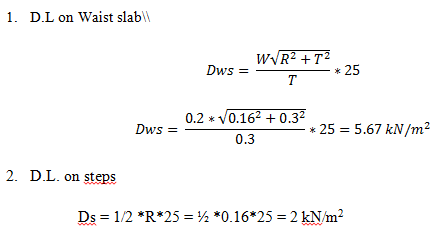
\includegraphics[width=10cm,height=10cm] {./images/stair d.png}
	
	\label{manual}
\end{figure}
Load per m on inclined stair slab W1, \\
W1 = Dws + Ds +L.L =12.67 kN/m\\
Load per m on landing slab W2,\\
W2 = W*25 + L.L = 0.2*25 + 5 = 10 kN/m\\
Maximum bending moment, M = 24.68 kNm\\
Factored Bending Moment, Mu¬¬ = 1.5 * 24.68 = 37.02 kNm\\
From IS 456, Annex G.1.1.c, Mu,lim > Mu , Hence safe\\
From Annex G.1.1.b\\
Mu = 0.87*fy*Ast*d*{1 – 0.42*fy /bdfck}\\
37.06*106           = 0.87*415*Ast(160-.42*.Ast/1000*30)\\ 
Asr                         = 680.922 mm2\\
Astmin                 =(0.12/100)*b*D\\ 
=192 mm2
Ast>Astmin\\
Provide 12 mm dia bars\\
Spacing             =140 mm\\
Provide 140 mm spacing\\

DISTRIBUTION REINFORCEMENT\\
Astmin                 = 192 mm2 \\
Provide 8 φ distributors @ 240c/c\\ 
CHECK FOR DEFLECTION\\
Ast,provided = 1583.363 mm2
Percentage of Tension, Pt = 100Ast,pro/bD = 0,395%\\
Modification factor for tension steel = 1.2 from Table 3 of IS456\\
Allowable L/d = 1.2 * 26 =31.2\\
Assumed L/d = 25, Hence OK\\
 \begin{figure}[H]
	
	\centering
	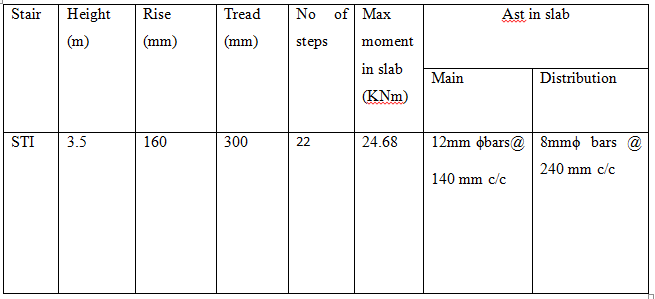
\includegraphics[width=\linewidth,height=6cm] {./images/stair.png}
	
	\label{manual}
\end{figure}

 \begin{figure}[H]
	
	\centering
	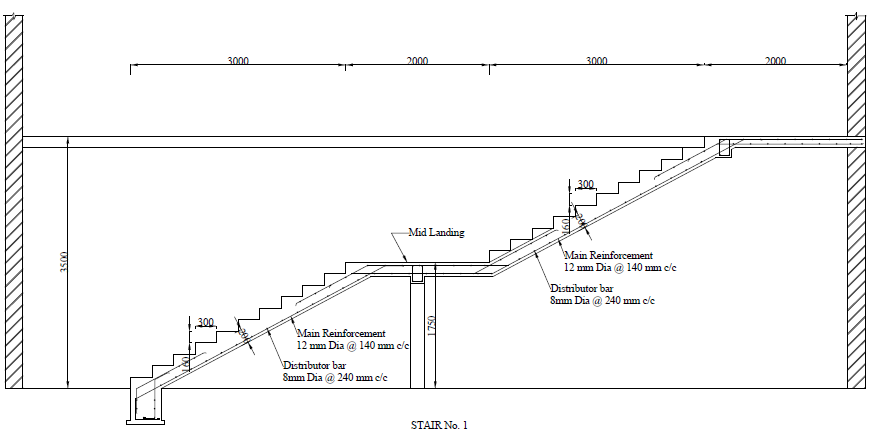
\includegraphics[width=\linewidth,height=10cm] {./images/stair1.png}
	
	\label{manual}
\end{figure}
\chapter{Estimate}
\section{General}
An estimate for any construction work may be defined as the process of calculating the quantities and costs of the various items required in connection with the work. It is prepared by calculating the quantities from the dimensions on the drawings for the various items required to complete the project and multiplied by unit cost of the item concerned. To prepare an estimate, drawings consisting of plan, elevation and the sections through important points are required.
\section{Methods of Estimation}
Estimate for a work or a project is necessary mainly for the purposes such as;
\begin{itemize}

\item	To ascertain the necessary amount of money required by the owner to complete the proposed work. 
\item	To ascertain quantities of materials required in order to programme their timely procurement. 
\item	To calculate the number of different categories of workers that are to be employed to complete the work within the scheduled time of completion.
\item	To assess the requirement of tools, plants and equipment required to complete the work according to the programme.
\item	To fix up the completion period from the volume of works involved in the estimate
\item	To draw up a construction schedule and programme and also to arrange the funds required according to the programme.
\item	To justify the investment from benefit-cost ratio.
\item	To invite tenders and prepare bills for payment.


\end{itemize}


\section{Methods of Taking Out Estimated}
The calculations of quantities of materials can be done using various methods of estimates. The application of an individual method depends upon the design and shape of the building. The different methods are as under:  \\
\begin{enumerate}
\item Centre line method\\ 
This method is suitable only if the offsets are symmetrical and the building is more or less rectangular in shape. The centre line of the building is determined carefully after doing deductions for repeated measurements (as explained in the next problem). This centre line acts as length for the complete calculations of the estimate. If the deduction is not cared for the results of estimates may be wrong. All the walls should have the same section. 
\item Crossing Method \\
In this method, lengths and breadths of the masonry walls at plinth level are taken (internal dimension of the room + thickness of the walls) for calculating quantities. The symmetrical offsets are a must as in the case of centerline method. 
\item Out to out and  in to in Method \\
  This method is most practicable under all circumstances and is generally followed in the P.W.D. for computing the quantities of various items. The estimation in this book has been done using this method. 
\item Bay Method \\
       This method is useful and is generally followed in case of building having several bays. The cost of the one class room is worked out and then multiplied by the number of bays in that building. The extra cost of the end walls and difference in framing. If there is any, should be made, so as to arrive at the correct cost. 
\item Service Unit Method. \\
This method is followed in cases such as school building where there are so many class rooms.  The cost of one class room us worked out and then multiplied by the number of class rooms to be constructed.   In case of Hospitals, the service unit is a bed, in case of Water Tank, it is a liter and in case of  Cinema Hall, the service unit is a seat.

\end{enumerate}
